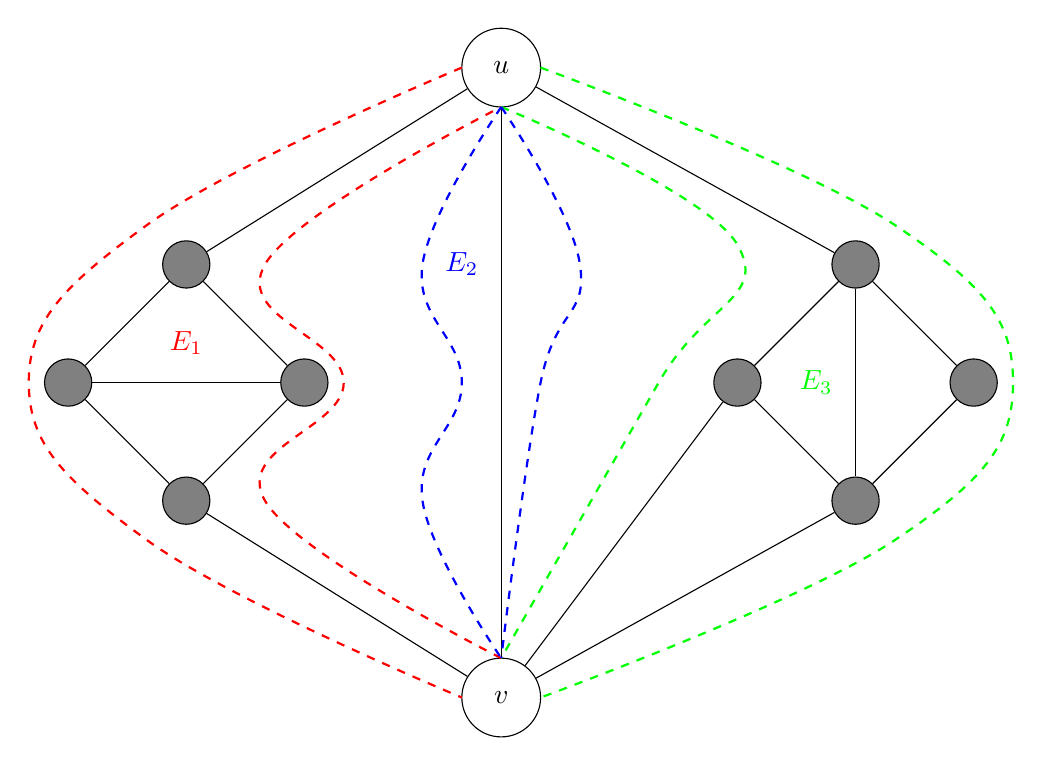
\begin{tikzpicture}

\node [circle, minimum height=1cm, draw] (v1) at (0,2.5) {$u$};
\node [circle, minimum height=1cm, draw] (v2) at (0,-5.5) {$v$};

\node [circle, minimum height=0.6cm, draw, fill=gray] (v3) at (-4,0) {};
\node [circle, minimum height=0.6cm, draw, fill=gray] (v4) at (-5.5,-1.5) {};
\node [circle, minimum height=0.6cm, draw, fill=gray] (v6) at (-2.5,-1.5) {};
\node [circle, minimum height=0.6cm, draw, fill=gray] (v5) at (-4,-3) {};

\node [circle, minimum height=0.6cm, draw, fill=gray] (v7) at (4.5,0) {};
\node [circle, minimum height=0.6cm, draw, fill=gray] (v10) at (3,-1.5) {};
\node [circle, minimum height=0.6cm, draw, fill=gray] (v8) at (6,-1.5) {};
\node [circle, minimum height=0.6cm, draw, fill=gray] (v9) at (4.5,-3) {};

\draw  (v1) edge (v2);

\draw  (v1) edge (v3);
\draw  (v3) edge (v4);
\draw  (v4) edge (v5);
\draw  (v5) edge (v6);
\draw  (v6) edge (v3);
\draw  (v5) edge (v2);
\draw  (v4) edge (v6);

\draw  (v1) edge (v7);
\draw  (v7) edge (v8);
\draw  (v8) edge (v9);
\draw  (v9) edge (v10);
\draw  (v10) edge (v7);
\draw  (v7) edge (v9);
\draw  (v9) edge (v2);
\draw  (v2) edge (v10);

\draw [dashed, thick, color=red] plot[smooth, tension=.7] coordinates {(-0.5,2.5) (-4.5,0.5) (-6,-1.5) (-4.5,-3.5) (-0.5,-5.5)};
\draw [dashed, thick, color=red] plot[smooth, tension=.7] coordinates {(0,-5) (-3,-3) (-2,-1.5) (-3,0) (0,2)};
\draw [dashed, thick, color=green] plot[smooth, tension=.7] coordinates {(0,2) (3,0.25) (2,-1.5) (0,-5)};
\draw [dashed, thick, color=green] plot[smooth, tension=.7] coordinates {(0.5,2.5) (5,0.5) (6.5,-1.5) (5,-3.5) (0.5,-5.5)};
\draw [dashed, thick, color=blue] plot[smooth, tension=.7] coordinates {(0,2) (-1,0) (-0.5,-1.5) (-1,-3) (0,-5)};
\draw [dashed, thick, color=blue] plot[smooth, tension=.7] coordinates {(0,2) (1,0) (0.5,-1.5) (0,-5)};
\node [color=red] at (-4,-1) {$E_1$};
\node [color=blue] at (-0.5,0) {$E_2$};
\node [color=green] at (4,-1.5) {$E_3$};
\end{tikzpicture}